\documentclass[a4paper]{article}

\usepackage[T1]{fontenc}              % Codificação para português 
\usepackage[brazilian]{babel}         % Português
\usepackage{hyphenat}                 % Use hifens corretamente
\usepackage{hyperref}                 % Links para páginas web
\usepackage{graphicx}                 % Figuras
\usepackage{float}                    % Figuras no lugar "esperado"
\graphicspath{{./images/}}            % Localização das imagens
\usepackage{fancyhdr}                 % Header estilo DCC
\setlength{\headheight}{24pt}

\title{Trabalho Prático I}
\author{Igor Lacerda Faria da Silva}
\date{\href{mailto:igorlfs@ufmg.br}{\texttt{igorlfs@ufmg.br}} }

\begin{document}

\pagestyle{fancy}
\lhead{Prof. Adriano Veloso

Aprendizado de Máquina}
\rhead{DCC / ICEx / UFMG 

2023.1}

\maketitle

\section{Introdução}
\label{sec:Introdução}

O objetivo deste trabalho é montar uma rede neural para identificar dígitos escritos à mão, a partir do banco de dados do \href{https://en.wikipedia.org/wiki/MNIST_database}{\texttt{MNIST}}. Este relatório compara diferentes variações dessa rede neural. A rede possui apenas 3 camadas e as variações exploram diferentes algoritmos, taxas de aprendizado e número de neurônios na camada oculta.

A comparação é dividida em 3 partes: inicialmente são fixados o algoritmo e a taxa de aprendizado, modificando-se o tamanho da camada oculta. Similarmente, a taxa é alterada e, por fim, o algoritmo. Conforme a especificação, os 3 algoritmos implementados foram: \textit{Stochastic Gradient Descent}, \textit{Gradient Descent} e \textit{Mini-Batch}. A implementação consistiu apenas em modificações de parâmetros simples da biblioteca.

A biblioteca utilizada foi o \href{https://www.tensorflow.org/}{\texttt{TensorFlow}}. Ela permite carregar diretamente o banco de dados do MNIST e possui uma \href{https://keras.io/api/}{\texttt{API}} conveniente para criar os modelos.

\section{Desenvolvimento}%
\label{sec:Desenvolvimento}

Foram analisadas duas métricas: a acurácia e a perda.

\subsection{Tamanho da Camada Oculta}%
\label{sub:Tamanho da Camada Oculta}

Foi fixada uma taxa de aprendizado $l_R = 1$ e um algoritmo de \textit{Mini-Batch}, com o tamanho da \textit{batch} igual a 50. A escolha desses parâmetros foi empírica: dentre as opções descritas no enunciado, o desempenho final da rede é intermediário.

\begin{figure}[H]
  \begin{center}
  {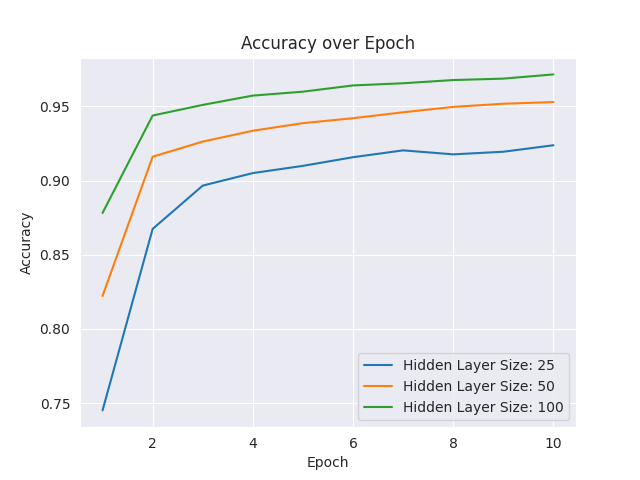
\includegraphics[height=7cm]{./images/Accuracy_over_Epoch_var_Hidden.png}}
  \end{center}
  \caption{Acurácia por época, variando o tamanho da rede. \label{fig:aeh}}
\end{figure}

\begin{figure}[H]
  \begin{center}
  {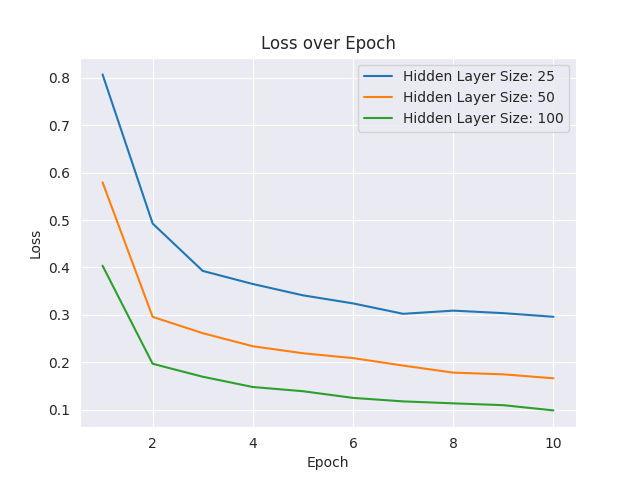
\includegraphics[height=7cm]{./images/Loss_over_Epoch_var_Hidden.png}}
  \end{center}
  \caption{Perda por época, variando o tamanho da rede. \label{fig:leh}}
\end{figure}

Como é de se esperar, o aumento do tamanho da rede melhorou a performance. Com mais neurônios é possível fazer ajustes mais sensíveis aos dados.

\subsection{Taxa de Aprendizado}%
\label{sub:Taxa de Aprendizado}

Foi fixada um tamanho de camada oculta igual a 50, e o algoritmo de \textit{Mini-Batch}, também com tamanho de \textit{batch} igual a 50. Novamente, a escolha desses parâmetros foi experimental, com base nas alternativas da especificação.

\begin{figure}[H]
  \begin{center}
  {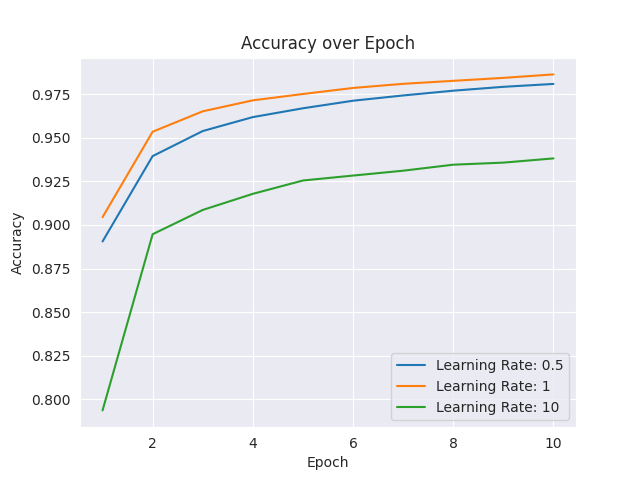
\includegraphics[height=7cm]{./images/Accuracy_over_Epoch_var_Rate.png}}
  \end{center}
  \caption{Acurácia por época, variando a taxa de aprendizado. \label{fig:aer}}
\end{figure}

\begin{figure}[H]
  \begin{center}
  {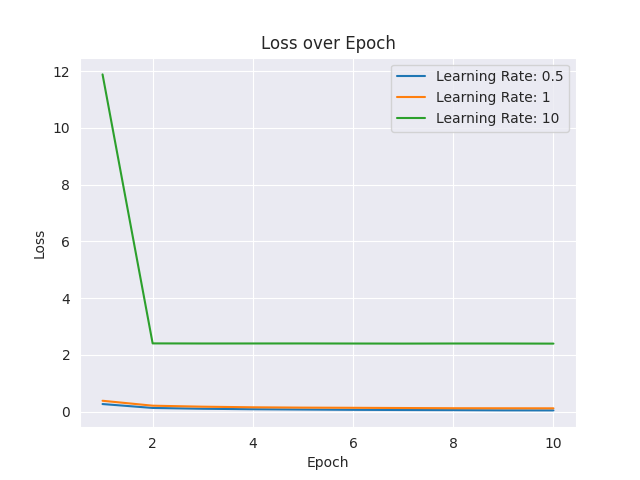
\includegraphics[height=7cm]{./images/Loss_over_Epoch_var_Rate.png}}
  \end{center}
  \caption{Perda por época, variando a taxa de aprendizado. \label{fig:ler}}
\end{figure}

Como visto em aula, uma taxa de aprendizado muito alta pode prejudicar a qualidade do modelo. Isso acontece porque a função de perda “pula” possíveis mínimos locais. Apesar de ter convergido nessa execução, o desempenho para a taxa igual a 10 não é diferente de um modelo que chuta que todos os dígitos são o número 9. Por outro lado, as taxas de 0.5 e 1, para essa execução, foram muito próximas em desempenho. No entanto, é comum que a taxa de 0.5 seja estatisticamente melhor. De fato, as taxas tradicionalmente usadas são muito menores do que as descritas na especificação: na faixa de 0.001 a 0.01. Por outro lado, uma taxa de aprendizado muito baixa também poderia aumentar o número de épocas para convergência.

\subsection{Algoritmo}%
\label{sub:Algoritmo}

As variações de algoritmo foram controladas alterando-se o parâmetro \textit{batch\_size}, da função \textit{fit()} do modelo. Em princípio, todos os algoritmos são o \textit{Mini-Batch}. Para criar um SGD, basta usar uma \textit{batch} de tamanho 1 e para criar um GD, é preciso usar uma taxa de aprendizado igual ao número de dados de treino. O número de épocas também precisou ser ajeitado: é preciso dar mais oportunidades de ajustes no GD, porque seus ajustes são muito infrequentes. Além disso, o tempo de execução do SGD é muito grande. Nos gráficos, o eixo $x$ representa o “progresso” do algoritmo (normalizado pelo número de épocas), cada ponto corresponde a uma época. A taxa de aprendizado, fixada em 1, e o número de neurônios, fixado em 50 foram escolhidos experimentalmente.

\begin{figure}[H]
  \begin{center}
  {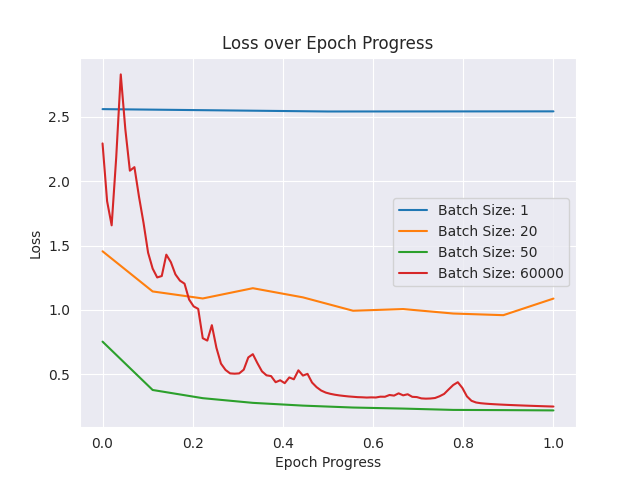
\includegraphics[height=7cm]{./images/Loss_over_Epoch_Progress.png}}
  \end{center}
  \caption{Acurácia por progresso em épocas, variando o algoritmo. \label{fig:lep}}
\end{figure}

\begin{figure}[H]
  \begin{center}
  {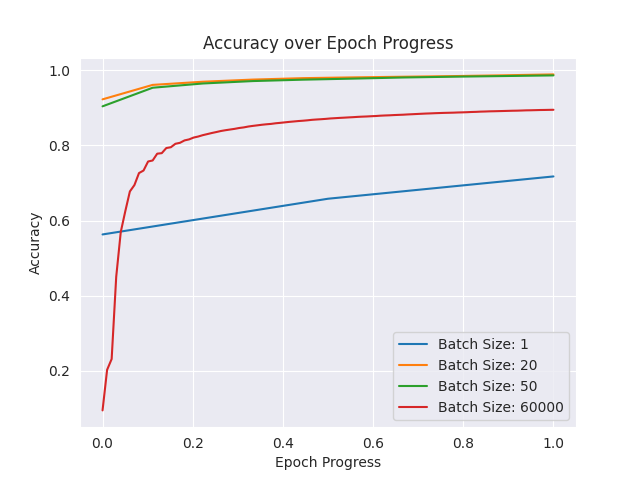
\includegraphics[height=7cm]{./images/Accuracy_over_Epoch_Progress.png}}
  \end{center}
  \caption{Acurácia por progresso em épocas, variando o algoritmo.\label{fig:aep}}
\end{figure}

O SGD teve um péssimo desempenho, também indiferente a apenas chutar algum número em particular. Como são feitos ajustes a cada dado, é como se o SGD “decorasse” o dado em questão. O GD, com 100 épocas, teve um desempenho similar ao MB (\textit{batch\_size = 50}). Com a diminuição do tamanho da \textit{batch}, o desempenho piorou consideravelmente. Uma provável causa para isso se deve aos ajustes dos pesos do modelo serem feitos de forma demasiadamente local, quando se considera apenas uma \textit{batch} com 20 dados.

\end{document}
